\documentclass[11pt]{article}
\usepackage[utf8]{inputenc}
\usepackage[english]{babel}
\usepackage{graphicx}
\usepackage{tabularx}
\usepackage{caption}
\usepackage[numbers]{natbib}

\graphicspath{{pics/}}

\DeclareUnicodeCharacter{00A0}{ }


\title{JSAI KDD Challenge 2001 (JKDD01) in WEKA \\ 4IZ451 - Knowledge discovery in databases}
\author{Tomáš Maršálek}
\date{\today}

\begin{document}
\maketitle
\thispagestyle{empty}
\clearpage

\section{Introduction}
Given a set of medical data of meningoencephalitis diagnoses we try to discover
predictive rules which could be used by domain experts to find out the cause of
the illness in various stages of diagnosis process (early symptoms, physical
examination and after laboratory results). We are also interested to find
similar rules to find out the culture of bacteria if the bacteria were the
cause in the first place. Lastly we are interested in prognosis of the patient
based on mentioned three stages of diagnosis process.

The analysis is performed using CRISP-DM methodology, which is a industry
standard method for data mining designed to perform vast data mining tasks
faster and more effectively while avoiding basic mistakes.


\section{CRISP-DM}
CRISP-DM (stands for CRoss Industry Standard Process for Data Mining) consists
of six stages from goal definition to results interpretation and deployment of
resulting model. The stages are:

\begin{enumerate}
    \item {\bf Business understanding} - The problem should be sufficiently understood so that it even makes sense to define goals
    \item {\bf Data understanding} - Data should be understood so that we understand meaning and quality of it
    \item {\bf Data preparation} - Models operate on data in a certain form. We preprocess the data to make the models digest the data properly and make the modeling as efficient as possible
    \item {\bf Modeling} - Various algorithms are performed to classify, segment, cluster, ... preprocessed data
    \item {\bf Evaluation} - Review the process done so far from step one because after obtaining more knowledge about the problem spending time working on it we should go back and see if we might have missed something or do something differently
    \item {\bf Deployment} - Presenting result of the analysis to the client if the goal was only to perform an analysis or implement the model programmatically to be used repeatedly by the client.
\end{enumerate}

\section{Goals}
The data mining challenge asks the analysts to find factors for
\begin{enumerate}
    \item diagnosis
    \item detection of bacteria or virus and culture of bacteria
    \item prognosis of the patient
\end{enumerate}

\section{Data}
Data set consists of 140 cases of patients with finding of severe inflammation
in dura mater (covering membrane of a brain).

The cases are described by 38 attributes from which we try to predict diagnosis
{\bf DIAG} and grouped diagnosis {\bf DIAG2} for the first goal of analysis.
For the second goal we are want to predict attributes {\bf CULT\_FIND} and {\bf
CULTURE} and to predict the prognosis of a patient we will use attributes {\bf
C\_COURSE} and {\bf COURSE}.


\mbox{}\\[.2cm]
\begin{table}[h]
\caption*{\bf Attributes known before physical examination - early symptoms}
\makebox[\textwidth][c]{
\begin{tabularx}{\textwidth}{|l|X|}
\hline
{\bf attribute} & {\bf explanation} \\
\hline
COLD & Days of symptoms of common cold \\
HEADACHE & Days of symptoms of headache \\
FEVER & Days of symptoms of fever \\
NAUSEA & Days of nausea \\
LOC & Days since loss of consciousness occured \\
SEIZURE & Days since convulsion or epilepsy observed \\
ONSET & - \\
\hline
\end{tabularx}
}
\label{tab:attrs_examination}
\end{table}

\mbox{}\\
\begin{table}[h]
\caption*{\bf Attributes known after physical examination}
\makebox[\textwidth][c]{
\begin{tabularx}{\textwidth}{|l|X|}
\hline
{\bf attribute} & {\bf explanation} \\
\hline
BT & Body temperature \\
STIFF & Neck stiffness \\
KERNIG & Kernig sign \\
LASEGUE & Lasegue sign \\
GCS & Glasgow Coma Scale \\
LOC\_DAT & Grouped loss of consciousness \\
\hline
\end{tabularx}
}
% \caption{}}
\label{tab:attrs_examination}
\end{table}


\mbox{}\\
\begin{table}[h]
\caption*{\bf Attributes known after laboratory tests}
\makebox[\textwidth][c]{
\begin{tabularx}{\textwidth}{|l|X|}
\hline
{\bf attribute} & {\bf explanation} \\
\hline
WBC & White Blood Cell Count \\
CRP & C-Reactive Protein \\
ESR & Blood Sedimentation Test \\
CT\_FIND & Grouped CT Findings \\
EEG\_WAVE & Grouped EEG Wave findings \\
EEG\_FOCUS & Focal sign in EEG \\
CSF\_CELL & Cell count in cerebulospinal fluid \\
Cell\_Poly & Polynuclear cell count in CSF \\
Cell\_Mono & Mononuclear cell count in CSF \\
CSF\_GLU & Glucose in CSF \\
CULT\_FIND & Whether bacteria or virus is specified or not \\
CULTURE & The name of bacteria or virus \\
\hline
\end{tabularx}
}
% \caption{}}
\label{tab:attrs_laboratory}
\end{table}


\mbox{}\\
\begin{table}[h]
\caption*{\bf Attributes after beginning of treatment}
\makebox[\textwidth][c]{
\begin{tabularx}{\textwidth}{|l|X|}
\hline
{\bf attribute} & {\bf explanation} \\
\hline
THERAPY2 & categorical type of therapy determined after diagnosis \\
CSF\_CELL3 & CSF after 3 days of treatment \\
CSF\_CELL7 & CSF after 7 days of treatment \\
C\_COURSE & Clinical course at discharge. Symptoms after discharge \\
COURSE & Grouped C\_COURSE. If symptoms found or not \\
RISK & Risk factor \\
\hline
\end{tabularx}
}
% \caption{}}
\label{tab:attrs_treatment}
\end{table}

\subsection{Data preprocessing}
Proprocessing steps for this analysis included finding columns with unknown
values and converting them into values recognizable by WEKA as unknowns (which
is symbol $?$).

Analysis is performed in stages as depicted in tables of attributes above.  For
each stage only attributes known in this or earlier stages are used to predict
attributes of following stages or goals. Therefore we end up with four
attribute-filtered data sets (early\_symptoms, examination, laboratory, treatment).

\section{Modeling}
WEKA of University of Waikato was used as a data mining tool for this analysis
for its simplicity, powerfulness and vast set of implemented classification
algorithms. Outstanding performance of algorithms is not needed due to size of
data set.

For the analysis we are interested only in classification rules which can be
reproduced by humans, eg.  to give a physician set of simple rules to determine
the cause of the illness and not to give him complex neural network which he
can not remember even though complex models will predict more accurately.
However because of the small sample size and huge amount of attributes this
problem is prone to overfitting. Therefore it doesn't even make sense to
compare complex classificators such as neural networks to simple rules and
pruned decision trees.

We first use algorithm One Rule which gives us insight and the most general
rule (no overfitting) for the predicted attribute. Success rate of this
classifier for this data set is often nothing to write home about though.
Next we use decision list algorithm PART\cite{Frank1998}\cite{weka_PART} which
is an algorithm that builds C4.5 decision tree to a limited depth. Result of
such a classifier is a set of simple rules which is perfect for our analysis.
Simpler rules that do not overfit as much are obtained with Ridor decision tree
algorithm. The most complex algorithm we use is J48, which is WEKA's implementation of
famous C4.5 decision tree algorithm. All of the decision tree based algorithms are pruned (reducedErrorPruning =
true).

We compare the models not by absolute error, but rather by Kappa statistic,
which tells us how much better relatively is the model to Zero Rule algorithm
(taking the majority class).



\section{Results}
After playing with the decision tree based classifiers and repeated
reevaluation after reprocessing data we got a set of rules that we will
present. Huge number of rules were obviously result of overfitting which we
tried to mitigate with post-prunning of the trees. We provide decision rules
found for each stage of diagnosis that we found general enough to be used by
domain experts.

\subsection{Early symptoms}
In a stage when a patient has not been examined by physician and only early
obvious symptoms can be observed, we haven't found any general rules that would
distinguish cause between bacterial and viral based only on symptoms of cold,
headache, fever, nausea, loss of consciousness, seizure and onset.

It follows that we haven't found any significant general rule to classify
culture of bacteria in case of bacterial cause based solely on early symptoms.
The most general rule was by One Rule algorithm with success rate of $24.24\%$.

Prognosis can't be predicted in this diagnosis stage either. No general rule
was found.

\subsection{Physical examination}
The patient was taken to a physician and routine diagnosis tests were
performed.

No general rule was found to predict diagnosis, however the closest one without overfitting is the
following set of rules by algorithm PART with overall success rate of $70.71\%$
and Kappa statistic $0.2882$.

\begin{verbatim}
SEX = F: VIRUS (44.0/5.0)

FEVER <= 11 AND
KERNIG <= 0 AND
FOCAL = - AND
AGE <= 62: VIRUS (19.0/1.0)

LASEGUE <= 0 AND
BT <= 39.7 AND
BT > 37.6: BACTERIA (14.0)

LOC_DAT = +: BACTERIA (10.0/3.0)
\end{verbatim}

Algorithm Ridor gives simpler rules for the cost of success rate ($67.14\%$) and kappa statistic ($0.1844$).
\begin{verbatim}
Diag2 = VIRUS  (140.0/42.0)
           Except (AGE > 45.5) and (BT > 37.85) and (FEVER <= 6.5) => Diag2 = BACTERIA  (9.0/0.0) [1.0/0.0]
\end{verbatim}


In order to predict whether culture is found, the best we can do is to use PART
to get success rate of $73.57\%$ and Kappa of $0.20$ at the cost of obvious
overfitting.

\begin{verbatim}
LOC_DAT = - AND
ONSET = ACUTE AND
COLD <= 8 AND
LOC <= 0 AND
FOCAL = - AND
LASEGUE <= 0 AND
SEX = F AND
AGE <= 51: F (22.0)

LOC_DAT = - AND
ONSET = ACUTE AND
COLD <= 8 AND
LASEGUE <= 0 AND
LOC <= 0 AND
FOCAL = - AND
SEX = M: F (33.0/4.0)

SEIZURE <= 1 AND
GCS > 10 AND
LOC_DAT = - AND
LASEGUE <= 0 AND
ONSET = ACUTE AND
COLD <= 4 AND
SEX = M: F (7.0)

SEIZURE <= 1 AND
GCS > 10 AND
ONSET = SUBACUTE: F (7.0/1.0)

SEIZURE <= 1 AND
GCS > 10 AND
LASEGUE > 0 AND
LOC_DAT = -: F (7.0)

SEIZURE <= 1 AND
GCS <= 10: F (6.0)

SEIZURE <= 1 AND
ONSET = ACUTE AND
BT > 39.6: T (5.0)

SEIZURE > 1: F (5.0)

ONSET = ACUTE AND
KERNIG > 0 AND
LOC <= 0: F (4.0)

ONSET = ACUTE AND
COLD > 4 AND
SEX = M: T (6.0)

FEVER <= 10 AND
ONSET = ACUTE AND
FEVER > 2 AND
BT <= 39.3: T (11.0/1.0)

ONSET = ACUTE AND
KERNIG <= 0 AND
FEVER > 0: F (12.0)

SEX = F AND
STIFF <= 0 AND
HEADACHE <= 9: T (3.0/1.0)

SEX = F: F (5.0)

FEVER <= 1: T (4.0)
\end{verbatim}

\section{Laboratory tests}
Results of laboratory examination are known and we have more attributes to use
to predict diagnosis, culture and prognosis.

Cause of meningoencephalitis can finally be generally predicted using attributes Cell\_Poly and Cell\_Mono without overfitting. PART found three simple rules with succes rate of $95.71\%$ and Kappa $0.899$.

\begin{verbatim}
Cell_Poly <= 220 AND
Cell_Mono > 12: VIRUS (96.0/1.0)

Cell_Poly > 3: BACTERIA (37.0)

CT_FIND = abnormal: BACTERIA (4.0)
\end{verbatim}

The same result is confirmed by Ridor algorithm with $93.57\%$ success rate and Kappa $0.844$.
\begin{verbatim}
Diag2 = BACTERIA  (140.0/98.0)
           Except (Cell_Poly <= 220.5) and (Cell_Mono > 7.5) => Diag2 = VIRUS  (67.0/1.0) [31.0/1.0]
\end{verbatim}






% \begin{figure}[!ht]
% 	\centering
% 	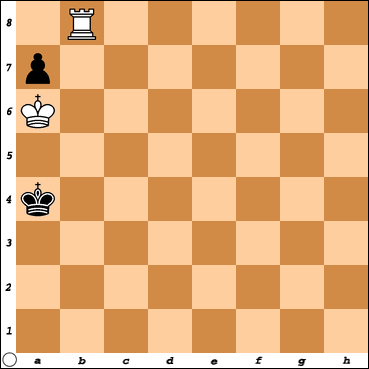
\includegraphics[width=.7\textwidth]{example}
% 	\caption{Example board setup}
%     \end{figure}
% 
% \clearpage

% \bibliographystyle{csplainnat}
% \bibliography{ref}

\end{document}
